\documentclass[11pt]{article}

\usepackage{latexsym}
\usepackage{amsmath}
\usepackage{amssymb}
\usepackage{amsthm}
\usepackage{graphicx}
\usepackage{wrapfig}
\usepackage{pseudocode}
\usepackage{url}
\usepackage{float}
\usepackage[backref, colorlinks=true, citecolor=red, urlcolor=blue, pdfauthor={Jyh-Ming Lien}]{hyperref}


\newcommand{\handout}[5]{
  \noindent
  \begin{center}
  \framebox{
    \vbox{
      \hbox to 5.78in { {\bf } \hfill #2 }
      \vspace{4mm}
      \hbox to 5.78in { {\Large \hfill #5  \hfill} }
      \vspace{2mm}
      \hbox to 5.78in { {\em #3 \hfill #4} }
    }
  }
  \end{center}
  \vspace*{4mm}
}

\newcommand{\lecture}[4]{\handout{#1}{#2}{#3}{#4}{#1}}

\newtheorem{theorem}{Theorem}
\newtheorem{corollary}[theorem]{Corollary}
\newtheorem{lemma}[theorem]{Lemma}
\newtheorem{observation}[theorem]{Observation}
\newtheorem{proposition}[theorem]{Proposition}
\newtheorem{definition}[theorem]{Definition}
\newtheorem{claim}[theorem]{Claim}
\newtheorem{fact}[theorem]{Fact}
\newtheorem{assumption}[theorem]{Assumption}

% 1-inch margins, from fullpage.sty by H.Partl, Version 2, Dec. 15, 1988.
\topmargin 0pt
\advance \topmargin by -\headheight
\advance \topmargin by -\headsep
\textheight 8.9in
\oddsidemargin 0pt
\evensidemargin \oddsidemargin
\marginparwidth 0.5in
\textwidth 6.5in

\parindent 0in
\parskip 1.5ex
%\renewcommand{\baselinestretch}{1.25}

\begin{document}

\lecture{Final Project Proposal: Automating Creation of Voting Districts}{Fall 2019}{William Austin}{CS 633 Computational Geometry}

\begin{abstract}

Investigate existing work and expand on current methods for automatic generation of voting districts.

\end{abstract}

\section{Motivation and Introduction}

Representative democracies, such as the United States, require voting populations to be grouped together into districts so that a single legislator can be elected to represent the interests of the people living within these boundaries. However, there are many different methods for creating these districts, and they are often prone to manipulation for political gain, a practice referred to as "gerrymandering". As more attention has been given to this problem in recent years, some progress has been made by requiring independent redistricting commissions in some states and deeming highly gerrymandered maps as illegal in the court system. In this project, we explore how algorithmic techniques could also be leveraged to alleviate many of these issues. 

We would like to be able to generate these districts programmatically using a predefined set of constraints, guaranteeing that the resulting maps are fair and unbiased, removing the influence of the political ambitions of the current party in power. Often, the negative effects of gerrymandering is summarized as "politicians picking their voters instead of voters picking their politicians."  However, the benefits of automating this process are more than creating politically neutral districts. It would also eliminate the manual effort needed to draw new boundaries, reducing costs.

Computationally, this is an interesting optimization problem, and there are several approaches that have been proposed for finding good solutions. We will focus on the method of "Balanced power diagrams", which is described in the referenced paper\cite{balanced_power_diagrams}. This approach seeks to optimize:
\begin{enumerate}
  \item Convexity of the district shape
  \item Minimal number of edges in each polygon representing the district
  \item Equal distribution of population across districts
\end{enumerate}

Some other measures that may be important include the ``compactness'' of the districts and the running time of the algorithm. For this project, I will use the methods pioneered by the researchers in the paper to generate potential districts based on the 2010 census data for Virginia. I have not reviewed the paper in depth, but the main technique seems to be reducing the problem to a graph representation and then computing a minimum cost flow.

\section{Methods to be Used and Studied}

As mentioned, I will be focusing on creating maps for Virginia. This includes:
\begin{enumerate}
  \item 11 Districts for the House of Representatives (US Congress)
  \item 40 Districts for the Virginia Senate (Upper House)
  \item 100 Districts for the Virginia House of Delegates (Lower House)
\end{enumerate}

In addition, I will provide some metrics for the generated districts. For example, the Polsby-Popper test is a measure of district compactness\cite{polsby_popper}. Brian Olson, a pioneer in this area, also computes average voter distance to the district center.\cite{brian_olson}

There is some sample code provided by the authors of the main paper\cite{balanced_power_diagrams}, which I plan on starting with and extending as needed. I am unsure of how complete the functionality is or how difficult will be to get it working. It is written in C++, which I also plan on using. In addition, like the original authors, I will be using data provided by the census for the computation\cite{census_data}.

As I mentioned, my primary focus is on the creation of maps for Virginia based on the techniques outlined in the paper.\cite{balanced_power_diagrams} However, if time permits, I will expand on the code. Some of the possibilities might be:
\begin{itemize}
  \item Compute maps for additional states.
  \item Modify the algorithm to optimize for other conditions.
  \item Introduce Monte Carlo techniques to speed up the algorithm.
\end{itemize}

\section{Gerrymandering Example}

\begin{figure}[H]
\centering
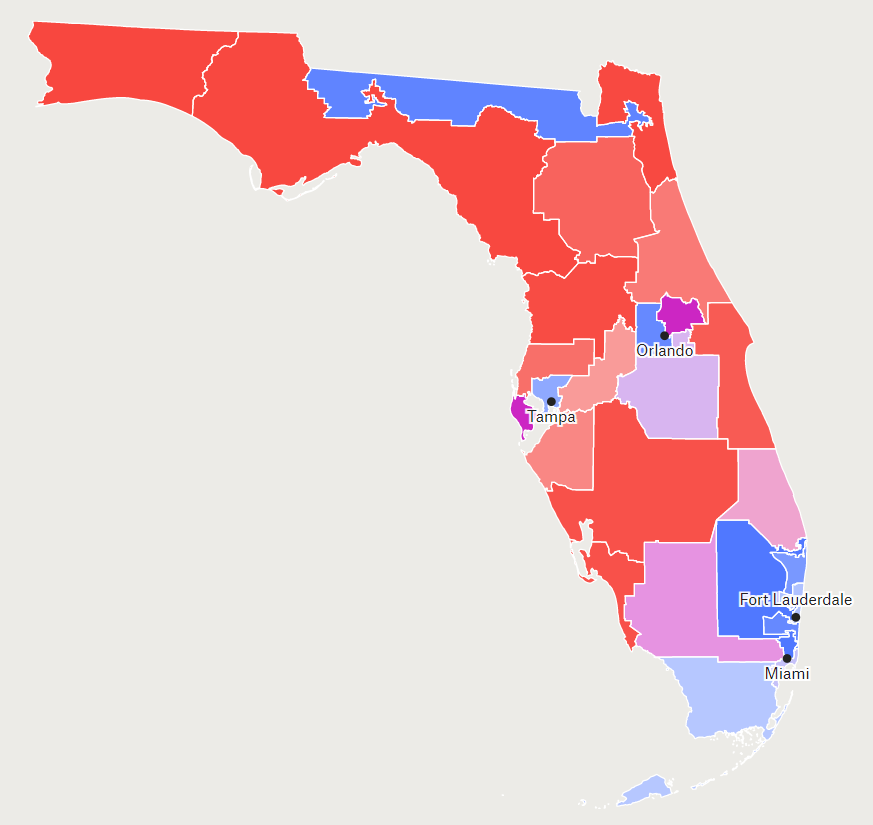
\includegraphics[scale=0.65]{FloridaCurrent.png}
\caption{Current Florida Congressional Districts\cite{florida_districts}}
\end{figure}

\begin{figure}[H]
\centering
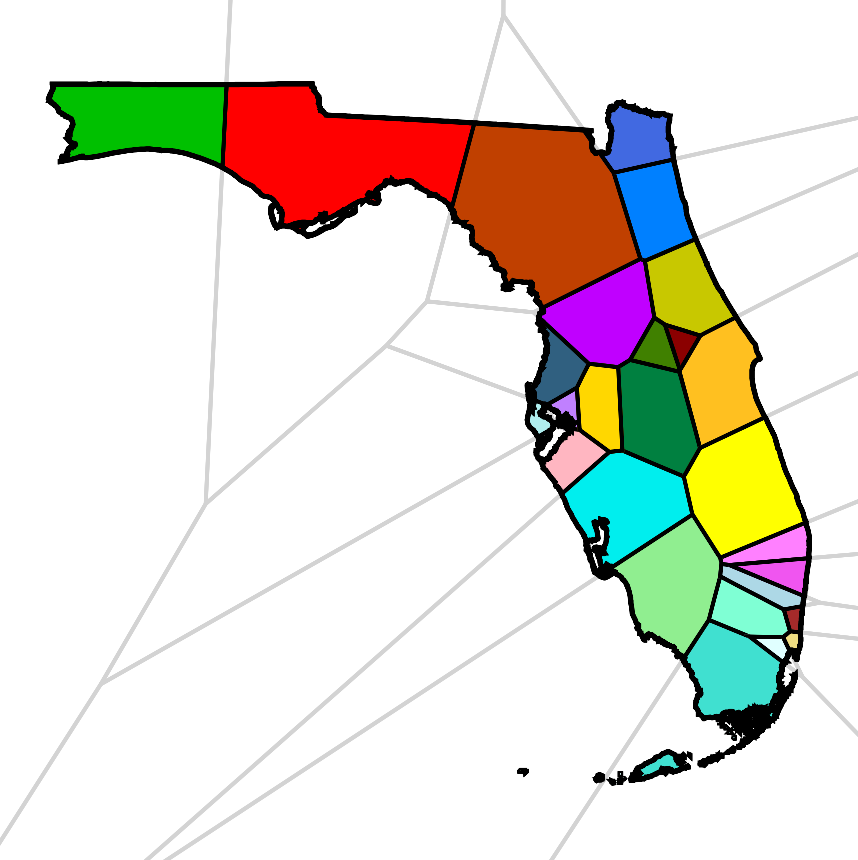
\includegraphics[scale=0.65]{FloridaNew.png}
\caption{Proposed Florida Congressional Districts}
\end{figure}

\begin{thebibliography}{999}

\bibitem{balanced_power_diagrams}
  Vincent Cohen-Addad, Philip N. Klein, and Neal E. Young. \emph{Balanced power diagrams for redistricting}, 2018.

\bibitem{polsby_popper}
  Polsby-Popper test. (n.d.). \emph{Wikipedia}. Retrieved October 15th, 2019, from \url{https://en.wikipedia.org/wiki/Polsby\%E2\%80\%93Popper_test}

\bibitem{brian_olson}
  Impartial Automatic Redistricting. (2010). \emph{Brian Olson's Website}. Retrieved October 15th, 2019, from \url{https://bdistricting.com/2010/}

\bibitem{florida_districts}
  Florida’s current congressional district boundaries. (2018). \emph{FiveThirtyEight: The Atlas Of Redistricting}. Retrieved October 15th, 2019, from \url{https://projects.fivethirtyeight.com/redistricting-maps/florida/}

\bibitem{census_data}
  United States Census Bureau. Cartographic boundary shapefiles -states. Retrieved October 15th, 2019, from \url{https://www.census.gov/geo/maps-data/data/cbf/cbf_state.html}.

\end{thebibliography}

\citation

\end{document}


